\chapter{Theoretical Background}
\label{chap:theory}

This chapter provides the theoretical foundation required to understand the contribution of this thesis. It first introduces the automotive context by defining \acp{HEV}, describing the main powertrain topologies, and outlining energy-management strategies with a focus on online learning-based control. The discussion then turns to simulation-based development and motivates the use of data-driven surrogate models as a computationally efficient alternative to high-fidelity physical vehicle simulations.

Building on this, the chapter introduces the machine-learning concepts needed later in the thesis. \acp{ANN} are presented as general nonlinear function approximators, followed by \acp{LSTM}s as a special type of \ac{ANN}s. The remainder of the chapter establishes the reinforcement-learning background: the agent--environment interaction, exploration and exploitation, \acp{MDP} and \acp{POMDP}, \ac{DRL}, and the actor--critic family of methods. The chapter concludes with the three specific algorithms used in this work, namely \ac{PPO}, \ac{TD3}, and \ac{SAC}.

\section{Hybrid Electric Vehicles}
\acp{HEV} are vehicles that use at least two distinct energy-transforming units and energy reservoirs for propulsion~\cite{world_forum_for_harmonisation_of_vehicle_regulations_wp29_mutual_2015}. Typically, those are represented by a chemical component (fuel) and an electrical component (battery). Whereas a conventional vehicle relies entirely on an \ac{ICE} for propulsion, an HEV integrates an \ac{EM} into the powertrain~\cite{kebriaei_hybrid_2015}.

The main purpose of hybridisation is to introduce an additional degree of freedom in how propulsion power is generated and distributed. This can reduce fuel consumption and generally improve vehicle efficiency~\cite{serrao_comparative_2011}. King and Nelson~\cite{king_model-based_2013} identified several mechanisms through which HEVs can reduce fuel consumption. The most important mechanisms are:

\begin{itemize}
  \item \textbf{Eliminating idle fuel use.} An \ac{HEV} can switch the engine off when no traction power is required and restart it rapidly when needed, thereby avoiding fuel consumption during engine-off standstill phases. This function is not exclusive to HEVs, since start--stop systems are also common in conventional vehicles, but hybridisation generally facilitates smoother and more frequent engine-off operation.
  \item \textbf{Recuperating braking energy.} During braking, a conventional vehicle wastes kinetic energy as heat, whereas an HEV can recover part of this energy and store it in a bidirectional energy storage system.
  \item \textbf{Downsizing the engine.} Since conventional vehicle engines are sized for peak demand but are often operated at partial load, HEVs can use electric machines to cover peak demand while allowing the \ac{ICE} to operate more frequently in higher-efficiency regions.
  \item \textbf{Improving engine operation.} In general, the additional degrees of freedom provided by electric integration enable the engine to operate in more efficient regions and can even facilitate electric-only driving. The extent of this benefit depends on the powertrain topology: series and power-split hybrids can decouple the \ac{ICE} operating point from the vehicle speed to a greater degree, whereas parallel hybrids retain a stronger mechanical link between engine speed and wheel speed~\cite{lin_progress_2024}.
\end{itemize}

Because improved fuel economy generally also reduces emissions, lower emissions are a further benefit of HEVs. However, although the mechanisms described above primarily target better fuel economy, fuel-consumption minimisation is not the main objective of this thesis. Instead, this work exploits the same additional control freedom to reduce tailpipe \ac{NOx} emissions while maintaining speed tracking and charge-sustaining operation.

\subsection{Classifying HEVs}
\acp{HEV} can be classified in several ways, such as by degree of hybridisation, by the nature of the power source, or by architecture and powertrain configuration~\cite{kebriaei_hybrid_2015}. The most relevant distinction for this thesis is the latter. The elementary hybrid powertrain topologies include series hybrids, parallel hybrids, and power-split hybrids~\cite{hofmann_hybridfahrzeuge_2023} (a schematic overview is provided in~\autoref{fig:hybrid-powertrains}):

\begin{itemize}
  \item \textbf{Series hybrid.} In a series hybrid system, the \ac{ICE} drives an electric generator instead of driving the wheels directly. In turn, the generator charges the battery and powers an electric motor that propels the vehicle. The electric motor is therefore the only unit directly coupled to the wheels~\cite{chan_electric_2010, enang_modelling_2017}.
  \item \textbf{Parallel hybrid.} In a parallel hybrid system, the \ac{ICE} and electric motor are both connected to a mechanical transmission in parallel. Both can therefore convert power into wheel motion~\cite{enang_modelling_2017}.
  \item \textbf{Power-split hybrid.} Also known as \emph{combined hybrid}, \emph{complex} or \emph{series-parallel}~\cite{kebriaei_hybrid_2015, enang_modelling_2017, chan_electric_2010}, these systems represent features of both, series and parallel hybrids. At the cost of higher complexity, this system can transfer power to the wheels mechanically, electrically, or through a combination of both paths. The central component is usually a planetary gearbox that mechanically couples the \ac{ICE} with the carrier gear, a first \ac{EM1} to the sun gear and the final driveshaft, and a second \ac{EM2} to the ring gear. This layout splits the power produced by the \ac{ICE} into a direct mechanical path to the wheels and an electrical path to charge the battery through a generator while enabling the \ac{ICE} speed to be independent of the vehicle speed~\cite{frey_data-based_2025}.

    \ac{EM1} functions as this generator when exerting negative torque on the sun gear~\cite{zhang_design_2015}. \ac{EM1} also controls the gear ratio and enables enables the continuously variable transmission. \ac{EM2} can provide additional torque on the ring gear or independently drive the vehicle electrically, depending on the exact architecture. Both electric motors can recuperate energy during braking~\cite{frey_data-based_2025}. A simple illustration of a planetary gearbox is depicted in~\autoref{fig:planetary_gearbox}.

    This high degree of freedom makes power-split hybrids efficient and adaptable, but it also increases component count, control complexity, manufacturing cost and vehicle mass~\cite{hofmann_hybridfahrzeuge_2023, frey_data-based_2025}.
\end{itemize}

\begin{figure}[htbp]
  \centering
  \begin{subfigure}[t]{0.62\textwidth}
    \centering
    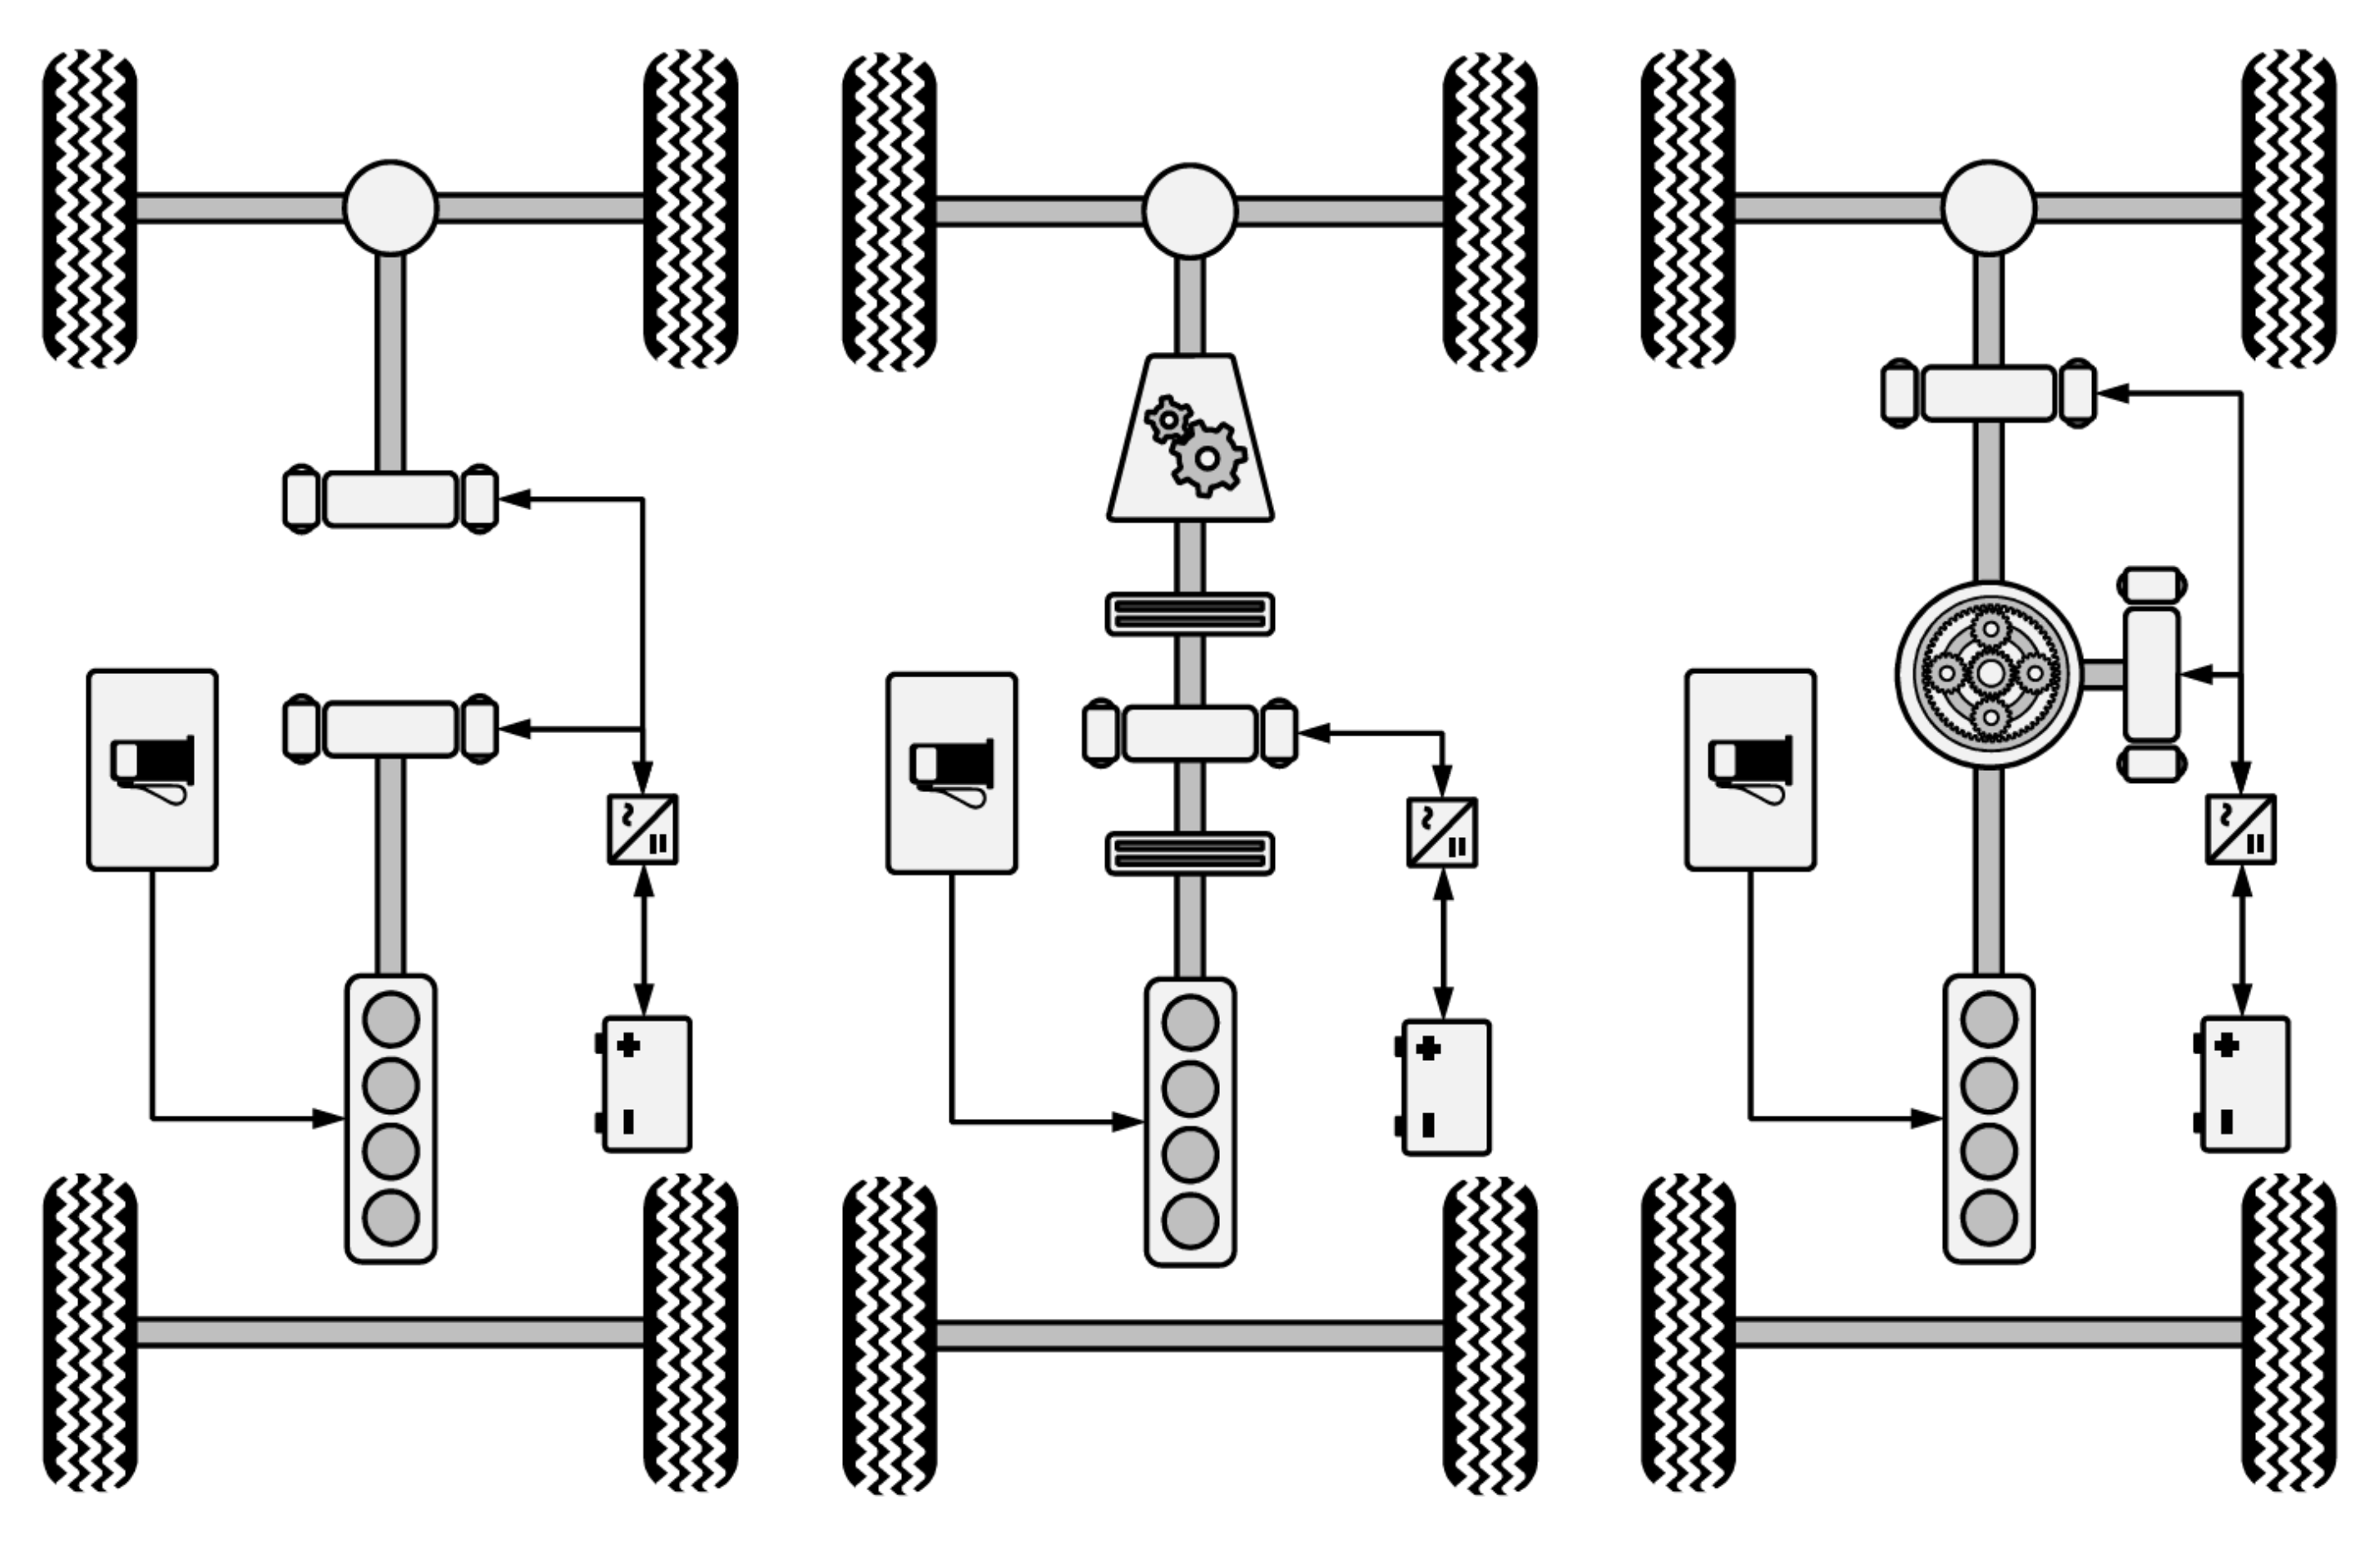
\includegraphics[width=\textwidth]{imgs/powertrains.png}
    \caption[Hybrid powertrain configurations]{Overview of the main hybrid powertrain configurations: series (left), parallel (middle), and power-split (right); reprinted from \cite{frey_data-based_2025}; original figures by \cite{casal_kulzer_grundlagen_2023}.}
    \label{fig:hybrid-powertrains}

  \end{subfigure}
  \hfill
  \begin{subfigure}[t]{0.32\textwidth}
    \centering
    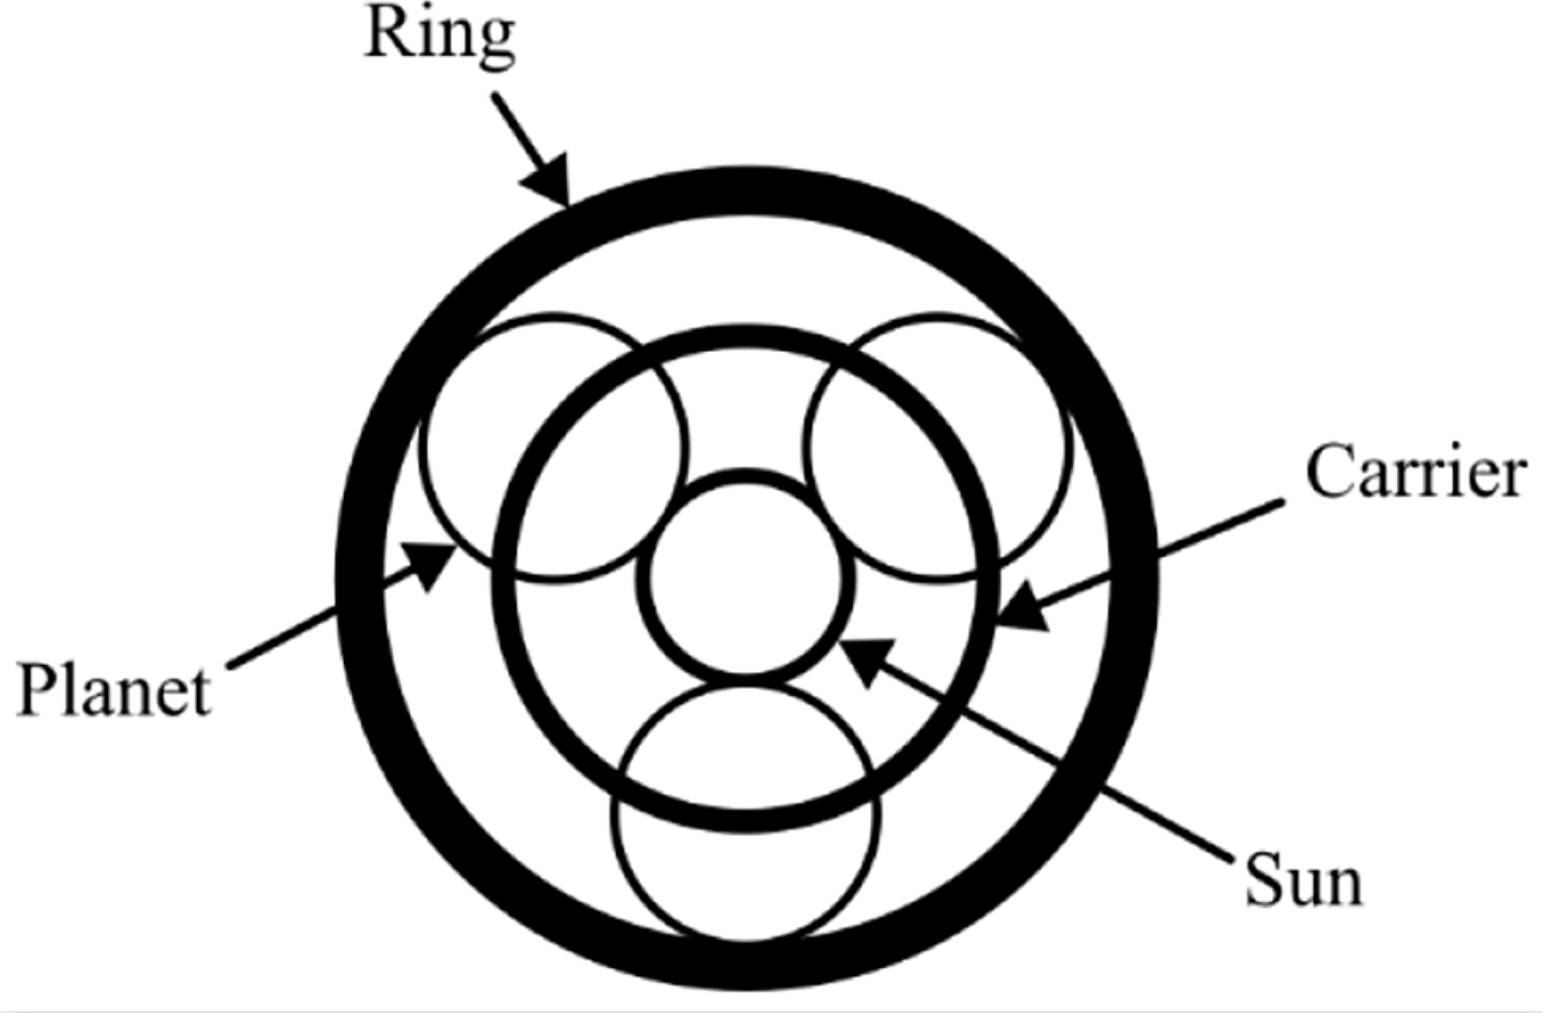
\includegraphics[width=\textwidth]{imgs/planetary_gear.png}
    \caption[Illustration of a planetary gearbox]{Illustration of a planetary gearbox; reprinted from \cite{frey_data-based_2025}.}
    \label{fig:planetary_gearbox}
  \end{subfigure}
  \caption[Hybrid powertrain configurations and planetary gearbox]{Hybrid powertrain configurations (left) and an illustration of a planetary gearbox (right).}
  \label{fig:hybrid_gearbox}
\end{figure}

\subsection{Control Strategies for HEVs}
Following the topology reported by Enang and Bannister~\cite{enang_modelling_2017}, \ac{HEV} energy management strategies can first be divided into \textit{offline} and \textit{online} approaches. This top-level distinction reflects whether the control policy is computed mainly before vehicle operation using a known drive cycle, or whether decisions are generated in real time while the vehicle is running. The individual strategy families and subcategories are summarised in~\autoref{fig:topology-control-strategies}.

\begin{figure}[htbp]
  \centering
  \includestandalone[width=\textwidth]{tikz/topology_control_strategies}
  \caption[Topology of HEV control strategies]{Topology of HEV control strategies. Artificial neural networks, which are used in this thesis through DRL are coloured; reprinted from~\cite{enang_modelling_2017}.}
  \label{fig:topology-control-strategies}
\end{figure}

\paragraph{Offline energy management strategies.}
Offline methods assume prior knowledge of the driving mission and therefore solve the energy management problem globally over a complete cycle. Their main purpose is to provide a performance benchmark and to quantify the best achievable fuel economy or emission performance under ideal information. However, their computational burden and their dependence on future driving information make them unsuitable for direct real-time implementation in production vehicles.

\paragraph{Online energy management strategies.}
Online strategies are designed for real-time use and therefore rely only on currently available data. For this thesis, the relevant point is the learning-based branch of the online taxonomy shown in~\autoref{fig:topology-control-strategies}. In particular, \ac{DRL} is attractive because it can learn policies from interaction data, can be applied to nonlinear black-box environments, and is suited to complex real-time optimisation tasks~\cite{tresca_cutting-edge_2025, zhou_self-learning_2022}.

\subsection{Simulation of HEVs}
\label{subsec:simulation_hevs}
As discussed above, DRL represents a promising control approach for the energy management of HEVs. As a control method that relies on \ac{ANN}s, it is inherently data-driven. Consequently, the availability of high-quality data is a fundamental prerequisite. Such data can be obtained either from measurements or from simulation of the vehicle dynamics. For simulation, two principal approaches exist: highly accurate physics-based simulations (often referred as digital twins), and surrogate models that approximate the original system with lower accuracy but higher sample efficiency~\cite{chakraborty_role_2021}. In engineering, Gamma Technologies' GT-SUITE~\cite{gamma_technologies_gt-suite_nodate} is widely used as a ``0D/1D'' simulator for modelling engines and drivetrains and enables the simulation of combustion, fluid flow, heat transfer, electrical components, and overall vehicle dynamics. However, because it must solve complex thermodynamic and fluid-dynamic equations, such simulations are typically slower than real time. For RL-based control strategies that rely on a vast amount of data, integrating such a simulator directly into the training loop is therefore not feasible. A promising alternative is data-driven modelling with \ac{ANN}s, especially \ac{LSTM}s, which are well suited for capturing the temporal dependencies that arise from drivetrain dynamics and thermally dependent emission aftertreatment (see~\autoref{subsec:thermal_state_complexity}). These models usually run much faster than high-fidelity physics-based simulations, but at the cost of accuracy. Nevertheless, because RL depends on large amounts of data, LSTM-based surrogate models provide a practical solution for this type of control problem; the central challenge is to find an appropriate trade-off between modelling accuracy and sample efficiency.

\subsection{The Complexity of the Thermal State}
\label{subsec:thermal_state_complexity}
Reducing tailpipe emissions in \acp{HEV} is more complex than minimising instantaneous fuel use or engine-out emissions. Diesel aftertreatment systems such as the \ac{DOC}, \ac{DPF}, and \ac{SCR} process exhaust gases downstream of the \ac{ICE}, but their effectiveness depends strongly on their thermal state. Below the light-off temperature, the catalyst is not yet sufficiently active and emissions generated by the engine may pass through the aftertreatment system with limited conversion. Consequently, an operating strategy that keeps engine load and exhaust temperature low at every instant is not necessarily optimal over a complete driving cycle. Temporarily operating the engine at a higher load can heat the aftertreatment system more rapidly and may reduce cumulative tailpipe emissions later in the cycle \cite{hofmann_hybridfahrzeuge_2023}.

This thesis does not treat aftertreatment control as a separate research objective. The short discussion is included to make the full control problem visible: the underlying vehicle model includes aftertreatment-related quantities such as \ac{SCR}, \ac{DOC}, and \ac{DPF} temperatures (see Appendix~\ref{app:model_interfaces}), and these temperatures depend on previous operation. This delayed thermal behaviour motivates the use of \acp{LSTM} as surrogate plant models (see~\autoref{subsec:simulation_hevs} and~\autoref{subsec:lstm_theory}) and helps explain why the real control problem is more accurately understood as a \ac{POMDP} (see~\autoref{subsec:current_limitations} and~\autoref{subsec:method_mdp}). For reasons of experimental feasibility, however, this thesis does not address the hidden thermal state with a recurrent \ac{RL} agent. This is further explained in \autoref{chap:methodology}.

\section{Artificial Neural Networks}
\label{sec:anns}
\ac{ANN}s, or \ac{NN}s, are machine-learning models that learn relationships between inputs and outputs from data. They were inspired by biological brains and consist of connected computational units, called neurons, that are arranged in layers. Each neuron combines incoming values with trainable weights and a bias and then applies a non-linear activation function. By stacking many such units, neural networks can approximate complex, non-linear relationships without manually defining all relevant features in advance~\cite{goodfellow_deep_2016}.

A typical feedforward network passes information from an input layer through one or more hidden layers to an output layer, as illustrated in~\autoref{fig:feedforward_ann}. During training, the network parameters are adjusted so that the predicted output becomes closer to a desired target. This is done by minimising a loss function, usually with mini-batch gradient-based optimisation and backpropagation. In practice, this means that prediction errors are propagated backwards through the network to determine how the weights should be updated. This flexibility makes \acp{ANN} suitable for prediction, function approximation and control tasks, but it also means that their performance depends strongly on the quality and coverage of the training data~\cite{goodfellow_deep_2016}.

\begin{figure}[htbp]
  \centering
  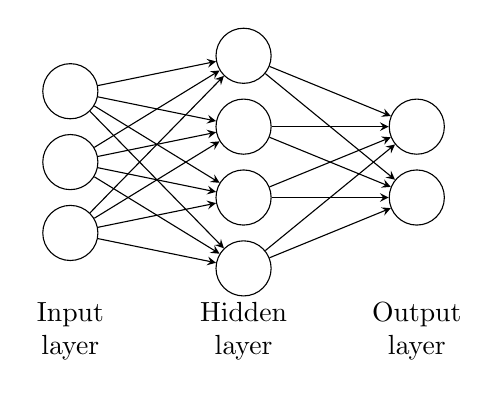
\begin{tikzpicture}[
      neuron/.style={circle, draw, minimum size=7mm},
      layerlabel/.style={align=center},
      connection/.style={->, >=stealth, thin}
    ]
    \foreach \i/\y in {1/0.9,2/0,3/-0.9} {
      \node[neuron] (I\i) at (0,\y) {};
    }
    \foreach \i/\y in {1/1.35,2/0.45,3/-0.45,4/-1.35} {
      \node[neuron] (H\i) at (2.2,\y) {};
    }
    \foreach \i/\y in {1/0.45,2/-0.45} {
      \node[neuron] (O\i) at (4.4,\y) {};
    }

    \foreach \i in {1,2,3} {
      \foreach \j in {1,2,3,4} {
        \draw[connection] (I\i) -- (H\j);
      }
    }
    \foreach \i in {1,2,3,4} {
      \foreach \j in {1,2} {
        \draw[connection] (H\i) -- (O\j);
      }
    }

    \node[layerlabel] at (0,-2.15) {Input\\layer};
    \node[layerlabel] at (2.2,-2.15) {Hidden\\layer};
    \node[layerlabel] at (4.4,-2.15) {Output\\layer};
  \end{tikzpicture}
  \caption[Feedforward neural network]{Simplified feedforward neural network with an input layer, one hidden layer and an output layer.}
  \label{fig:feedforward_ann}
\end{figure}

\subsection{Long Short-Term Memory}
\label{subsec:lstm_theory}
\acp{LSTM} are a special type of \ac{RNN} introduced by Hochreiter and Schmidhuber \cite{hochreiter_long_1997}. Unlike feedforward networks, which process each input independently, recurrent networks maintain an internal state that is updated over time. This makes them suitable for sequential data, where the current output depends not only on the current input but also on previous operating conditions \cite{goodfellow_deep_2016}.

The main idea of an \ac{LSTM} is to extend the recurrent state with a memory cell. As shown in \autoref{fig:lstm_cell}, this memory is regulated by gates: a forget gate determines which previous information should be retained, an input gate controls how much new information is written, and an output gate determines which part of the memory is exposed to the next layer or time step. This gated structure helps \acp{LSTM} preserve relevant temporal information over longer horizons than conventional recurrent networks \cite{goodfellow_deep_2016, hochreiter_long_1997}.

\begin{figure}[htbp]
  \centering
  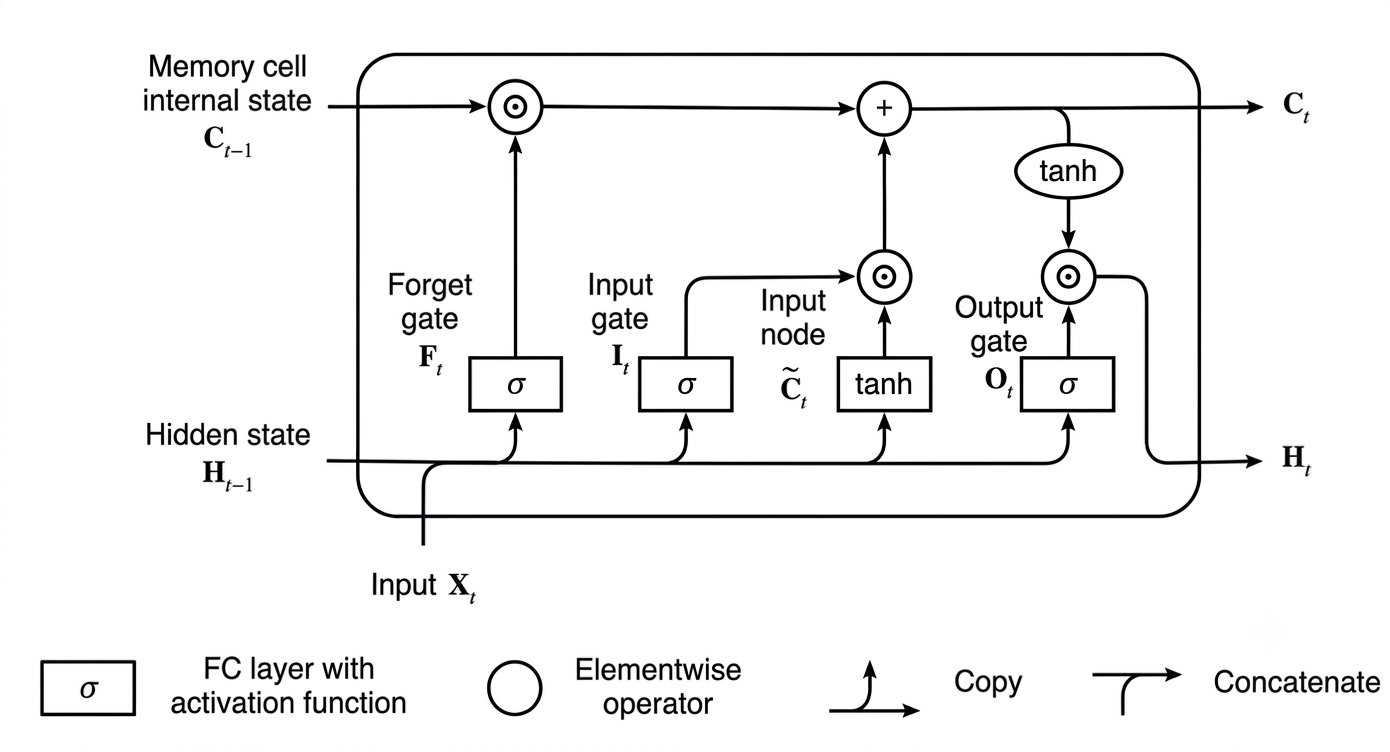
\includegraphics[width=0.6\textwidth]{imgs/lstm_cell.png}
  \caption[LSTM cell structure]{Structure of an LSTM cell showing the memory path and the gates that regulate the flow of temporal information; adapted from \cite{zhang_dive_2023}.}
  \label{fig:lstm_cell}
\end{figure}

In the context of this thesis, \acp{LSTM} are relevant because the hybrid powertrain behaviour cannot be described reliably from the instantaneous input alone. Specifically the internal temperatures of the system inherit a temporal lag which makes them highly dependent on previous operating points. LSTM-based surrogate models can therefore capture dynamic relationships in the simulated vehicle while remaining much faster to evaluate than high-fidelity physical simulations (see \autoref{subsec:simulation_hevs}). In this work, the \acp{LSTM}s are used for the surrogate environment, whereas the \ac{RL} agents themselves are implemented in their non-recurrent version (see \autoref{chap:methodology}).

\section{Reinforcement Learning}
Besides supervised and unsupervised learning, \ac{RL} is commonly representing the third pillar of machine learning. In contrast to the former two, which rely on pre-collected datasets, \ac{RL} is based on sequential interaction between a learning agent and an environment \cite{sutton_reinforcement_2020}.

To formalise \ac{RL}, several elements are necessary:

\begin{itemize}
  \item \textbf{Agent.} The agent is the decision-making entity in reinforcement learning. It observes the available information from the environment, selects actions, and improves its behaviour over time based on the feedback it receives.
  \item \textbf{Environment.} The environment represents everything external to the agent with which it interacts. It responds to the agent's actions by changing its state and by returning new observations and rewards.
  \item \textbf{Policy.} A policy defines the agent's behaviour by specifying which action should be chosen in a given situation. It can be deterministic or stochastic and represents the object that the agent ultimately tries to optimise.
  \item \textbf{Reward signal.} The reward signal is a scalar feedback value that evaluates the immediate consequence of an action. It defines the learning objective by indicating which behaviours are desirable and which should be avoided.
  \item \textbf{Value function.} The value function estimates how beneficial a state or state--action pair is in the long term. In this way, it supplements the immediate reward by capturing the expected cumulative future return.
  \item \textbf{Model of the environment.} A model describes how the environment evolves and what rewards are likely to result from actions. Such a model is optional since model-free \ac{RL} exists; the algorithms considered in this thesis do not require an explicit model of the transition dynamics.
\end{itemize}

At each time step, the agent observes the current situation, selects an action, and receives feedback from the environment in the form of a reward. The objective of the agent is to learn a policy that maximises the expected cumulative reward over time. An illustration of the \ac{RL} interaction loop is depicted in \autoref{fig:agent-environment-rl} \cite{sutton_reinforcement_2020}.

\begin{figure}[htbp]
  \centering
  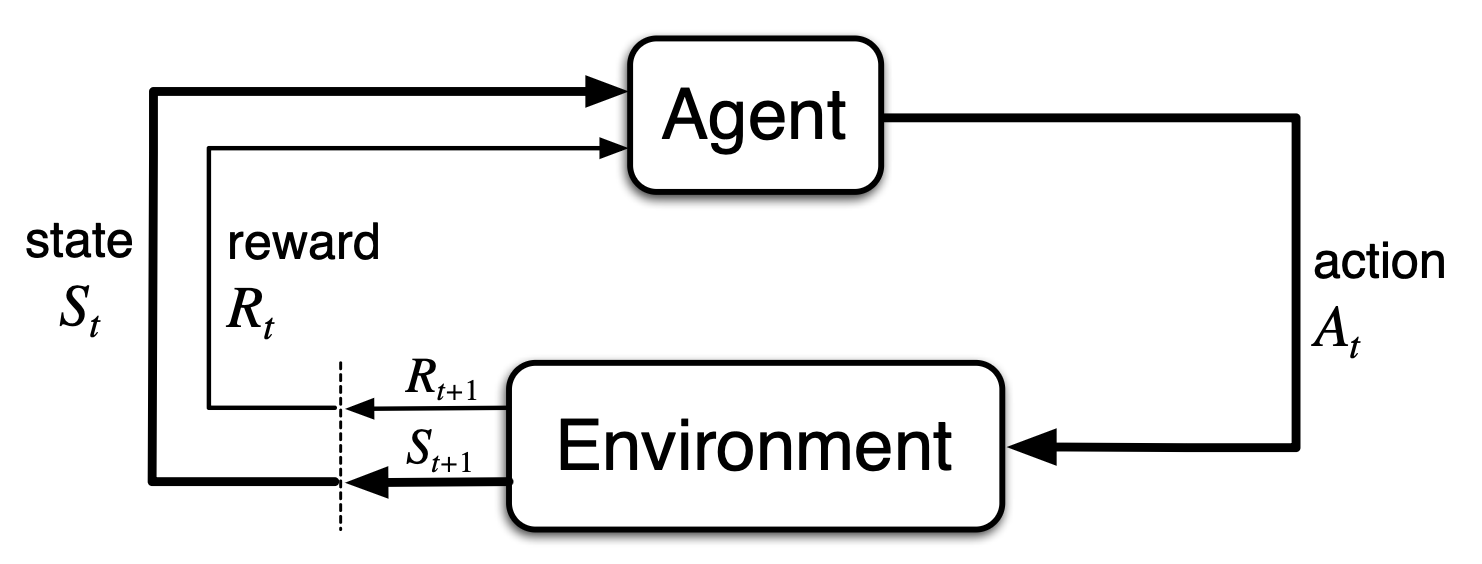
\includegraphics[width=0.45\textwidth]{imgs/agent_environment.png}
  \caption[Agent--environment interaction]{Agent--environment interaction in a Markov decision process; reprinted from \cite{sutton_reinforcement_2020}.}
  \label{fig:agent-environment-rl}
\end{figure}

\paragraph{Exploration versus exploitation.}
The central challenge in \ac{RL} is the trade-off between exploration and exploitation. On the one hand, the agent must exploit behaviours that already appear promising in order to maximise cumulative reward. On the other hand, it must continue to explore alternative actions so that potentially better solutions are not overlooked too early. The difficulty is that an agent cannot focus exclusively on only one of these two objectives without impairing learning performance. This dilemma represents the \emph{fundamental challenge} in \ac{RL} \cite{sutton_reinforcement_2020}.

\subsection{Markov Decision Process}
The standard mathematical framework used to formulate reinforcement-learning problems is the Markov Decision Process, \ac{MDP}. It can be described as a sequential decision problem by the tuple $(\mathcal{S}, \mathcal{A}, P, R)$, where $\mathcal{S}$ denotes the state space, $\mathcal{A}$ the action space, $P(s_{t+1}\mid s_t, a_t)$ the state-transition probability, and $R(s_t, a_t, s_{t+1})$ the reward function \cite{hausknecht_deep_2017}. At each time step $t$, the agent is in state $s_t \in \mathcal{S}$, chooses an action $a_t \in \mathcal{A}$, transitions to a new state $s_{t+1}$ according to the dynamics $P$, and receives a scalar reward. Different authors use slightly different conventions for this tuple: some include a discount factor $\gamma$ \cite{ni_recurrent_2022}, which weights the relevance of future rewards, while others define an \ac{MDP} through a four-argument probability function \cite{sutton_reinforcement_2020}.
The defining property of an \ac{MDP} is the \emph{Markov property}, which states that the transition probabilities fully encode the environment's dynamics. Consequently, the probability of the next state depends only on the current state--action pair $(s_t, a_t)$ and not on the history of previous states and actions \cite{sutton_reinforcement_2020}:

\begin{equation}
  P(s_{t+1} \mid s_t, a_t, s_{t-1}, a_{t-1}, \dots, s_0, a_0)
  =
  P(s_{t+1} \mid s_t, a_t).
\end{equation}

In many real-world applications, however, the true system state is not fully observable. Instead, the agent only has access to incomplete, noisy, or indirect observations. Such problems are more appropriately described by a partially observable MDP, \ac{POMDP}. In this case, the agent receives an observation $o_t$ rather than the full state $s_t$, so the Markov property does not necessarily hold for the observation alone. This makes the decision problem more difficult, because the agent must infer relevant information about the hidden state from the observation history \cite{sutton_reinforcement_2020}.

The distinction between \acp{MDP} and \acp{POMDP} is highly relevant in practice. Many control problems are modelled as \acp{MDP} for simplicity, even though the available measurements do not fully describe the underlying system. In these cases, a suitable state representation, history window, or recurrent model can help approximate the missing information. This is one reason why sequence models such as \acp{LSTM} can be useful in reinforcement learning settings: they help encode temporal context when the current observation is insufficient to characterise the environment completely \cite{sutton_reinforcement_2020, ni_recurrent_2022, hausknecht_deep_2017}.

\subsection{Deep Reinforcement Learning}
Foundational \ac{RL} methods are often introduced in tabular form. In this setting, value functions, policies, or both are represented explicitly as tables whose entries correspond to individual states or state--action pairs. Such formulations are the most basic representation of \ac{RL}, but they become impractical as soon as the control problem grows in complexity \cite{sutton_reinforcement_2020}.

The main limitation is scalability. If the state space or action space is continuous, it must first be discretised before a table can be used. This introduces approximation errors and, depending on the granularity of the discretisation, can also lead to an enormous number of table entries. The same issue appears in high-dimensional problems where the number of possible state combinations grows combinatorially, making \ac{RL} prohibitively expensive or unfeasible \cite{lillicrap_continuous_2019, sutton_reinforcement_2020}.

A solution is to replace explicit tables with function approximators. Instead of storing a separate value for every individual state or action, the agent learns a parametric function that maps observations or state--action pairs to value estimates, policies, or both. This allows the agent to generalise from observed samples to unseen states and actions, and to operate in spaces that are too large for explicit enumeration. Among the available function approximators, \acp{NN} have proven especially powerful (see \autoref{sec:anns}). In \ac{RL}, \acp{NN} can therefore be used to approximate value functions, policies, or complete actor--critic architectures \cite{sutton_reinforcement_2020}.

\ac{DRL} is exactly this combination of \ac{RL} with deep \ac{NN} function approximation. It makes \ac{RL} applicable to high-dimensional, continuous, and nonlinear problems that would otherwise be intractable. In the context of this thesis, this step is essential because the considered \ac{HEV} control task involves continuous control actions, nonlinear vehicle and aftertreatment dynamics, and observations whose relevance can depend on temporal context. A neural-network policy or critic can operate directly on such continuous representations and can be trained from simulated interaction data without manually enumerating the state--action space~\cite{lillicrap_continuous_2019, sutton_reinforcement_2020}. In the following, \ac{RL} and \ac{DRL} are used interchangeably because the deep variant is the only form used in this work.

\subsection{Classifying RL Algorithms}
The following taxonomy is intentionally non-exhaustive. Its purpose is not to cover every family of \ac{RL} algorithms, but to introduce the distinction that leads to the actor--critic methods used in this thesis. A useful starting point is the pair of classical algorithmic viewpoints of \emph{value iteration} and \emph{policy iteration}. Although modern \ac{DRL} algorithms are usually formulated with neural-network function approximators rather than explicit tables, these two perspectives still provide the conceptual basis for classifying many \ac{RL} methods~\cite{sutton_reinforcement_2020}.

\paragraph{Value-based methods.} In value-based methods, the central object of learning is a value function, for example a state-value function $V(s)$ or an action-value function $Q(s,a)$. The policy is obtained only indirectly from these estimates by selecting the action with the highest predicted return. Learning therefore focuses on evaluating the long-term consequences of actions first, while decision-making follows from this evaluation step \cite{sutton_reinforcement_2020}.

\paragraph{Policy-based methods.} In policy-based methods, the policy itself is the object of optimisation. Instead of deriving behaviour from value estimates, a parameterised policy $\pi_{\theta}(a \mid s)$ is adjusted directly so that the expected discounted return
\begin{equation}
  G_t = \sum_{k=0}^{\infty} \gamma^k r_{t+k+1}
\end{equation}
is maximised. This perspective is particularly attractive in continuous-action problems, because it avoids the need to search over all possible actions, and it naturally permits stochastic policies. For this reason, direct policy optimisation plays a central role in modern continuous-control DRL \cite{sutton_reinforcement_2020, lillicrap_continuous_2019}.

\paragraph{Actor--critic methods.} These arise as a synthesis of these two families. The actor represents the policy and selects actions, while the critic estimates a value function that assesses the quality of states, actions, or the current policy. The critic thereby provides a training signal for improving the actor, whereas the actor generates the behaviour from which the critic learns. Actor--critic approaches can thus be interpreted as combining the direct optimisation of policy-based methods with the evaluative structure of value-based methods \cite{barto_neuronlike_1983, sutton_reinforcement_2020}. This combination is especially important in \ac{DRL}, where it often improves data efficiency and stabilises learning in high-dimensional and continuous domains.

\begin{figure}[htbp]
  \centering
  \includestandalone[width=0.8\textwidth]{tikz/rl_tax}
  \caption[Taxonomy of RL algorithms]{A non-exhaustive, but useful taxonomy of algorithms in modern RL; algorithms used in this thesis are coloured; adapted from~\cite{openai_part_nodate}.}
  \label{fig:rl_taxonomy}
\end{figure}

This taxonomy is useful for positioning the algorithms discussed later, since all three methods considered in this work are actor--critic algorithms and therefore inherit characteristics from both direct policy optimisation and value-function learning (\autoref{fig:rl_taxonomy}).

\subsection{Overview of Actor--Critic Architectures}
\label{subsec:actor-critic-architectures}
Building on the taxonomy above, actor--critic architectures combine value-based and policy-based learning within a single framework. They learn a parameterised policy $\pi_{\theta}(a \mid s)$ and a value function, such as $V(s)$ or $Q(s,a)$, at the same time \cite{sutton_reinforcement_2020}.

This combination addresses several limitations of the two individual paradigms by using two interacting sets of neural-network parameters:

\begin{itemize}
  \item \textbf{The actor.} Represents the policy parametrisation, $\theta$. It determines the agent's behaviour by mapping states to actions. The actor's weights are updated in the direction suggested by the critic so that the expected return is increased.
  \item \textbf{The critic.} Represents the value-function parametrisation $\omega$. It evaluates the actions taken by the actor and provides a learning signal for improving the current policy.
\end{itemize}
Actor--critic methods address key limitations of purely value-based and purely policy-based reinforcement learning by combining their main strengths within a single architecture. A simple illustration of an actor--critic architecture is depicted in \autoref{fig:actor-critic-loop}.

\paragraph{Limitations of value-based methods.}
Purely value-based methods are often comparatively sample-efficient, but they are less natural for continuous action spaces and for learning genuinely stochastic policies. In such settings, selecting an action by maximising a value function over all possible actions becomes difficult or even intractable. Actor-based parameterisations avoid this problem by learning the parameters of a policy distribution directly, for example the mean and standard deviation of a Gaussian distribution \cite{sutton_reinforcement_2020, lillicrap_continuous_2019}.

\paragraph{Limitations of policy-based methods.}
Purely policy-based methods are well suited to continuous control because they optimise a parameterised policy directly. However, they often suffer from high-variance gradient estimates because they rely on sampled trajectory returns. In the classical REINFORCE algorithm, for example, the return is estimated with Monte Carlo sampling. This means that the complete realised return of a trajectory is used as the learning signal, so an update may have to wait until the end of an episode and can vary strongly between sampled trajectories. Although such estimates are unbiased, they can therefore lead to slow and unstable learning. Actor--critic methods reduce this variance by introducing a critic that bootstraps value estimates and enables temporal-difference learning. Bootstrapping means that the current value estimate is updated from an immediate reward plus the critic's estimate of the next state, for example through a target of the form $r_{t+1} + \gamma V(s_{t+1})$. This introduces some bias, but it provides stepwise feedback on the actor's decisions and usually yields a lower-variance training signal \cite{sutton_reinforcement_2020}. Modern actor--critic methods often refine this idea further by using the advantage function, $A(s,a) = Q(s,a) - V(s)$, so that the critic evaluates how much better an action is compared with the baseline value of the state. This usually yields a more stable and informative learning signal for policy updates \cite{schulman_proximal_2017}.

\paragraph{Data efficiency via off-policy learning.}
A further advantage of many actor--critic architectures is that they can be combined with off-policy learning. Whereas basic on-policy methods can only learn from data generated by their current target policy, off-policy methods improve a \emph{target policy} while using a different \emph{behaviour policy} to generate data \cite{sutton_reinforcement_2020}. This can substantially improve data efficiency because collected experience remains useful even after the policy has been updated.

In practice, this is commonly realised with an experience replay buffer, which stores interactions with the environment as transition tuples of the form $(S_t, A_t, R_{t+1}, S_{t+1})$. This idea was introduced by Lin \cite{lin_self-improving_1992} under the term \emph{experience replay}. By sampling from this buffer, the agent can reuse past experience in mini-batch updates rather than updating only from the most recent transition. This improves computational efficiency and leads to more stable gradient estimates. In addition, random sampling from the replay buffer breaks the strong temporal correlations that are present in consecutive samples from a trajectory, which can further stabilise learning \cite{lillicrap_continuous_2019}. For the present work, this distinction is important because \ac{PPO} is an on-policy method, whereas \ac{TD3} and \ac{SAC} are off-policy methods that can exploit replay buffers.

\begin{figure}[htbp]
  \centering
  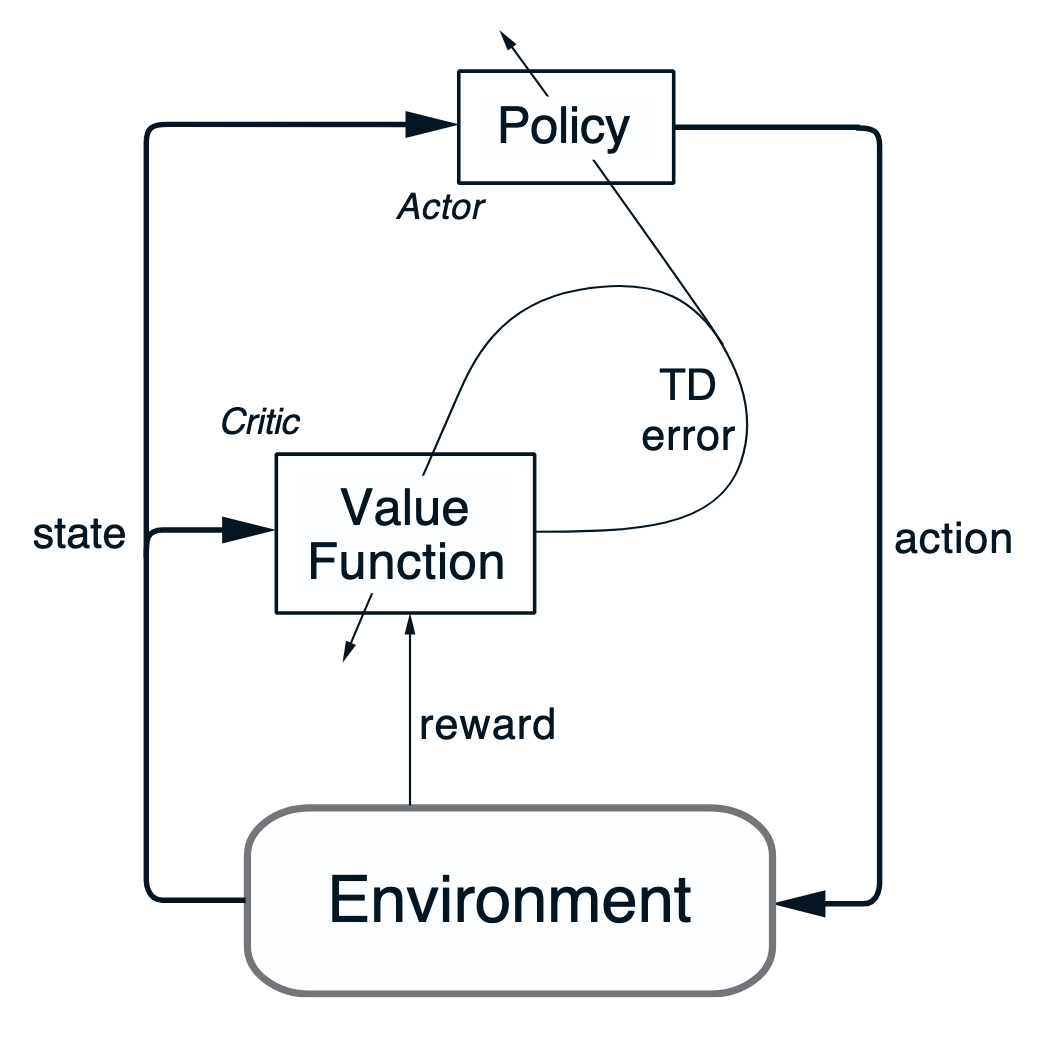
\includegraphics[width=0.35\textwidth]{imgs/actor_critic.png}
  \caption[Actor--critic architecture]{The actor--critic architecture; reprinted from \cite{s_sutton_reinforcement_2014}.}
  \label{fig:actor-critic-loop}
\end{figure}

The three algorithms used in this thesis all belong to the actor--critic family. They differ along two main axes: \ac{PPO} is on-policy with a stochastic policy, \ac{TD3} is off-policy with a deterministic policy, and \ac{SAC} is off-policy with a stochastic policy regularised by an entropy term. The selection rationale is given in \autoref{subsec:method_algo_selection}; the present subsections only summarise their algorithmic mechanics.

\subsection{Proximal Policy Optimisation (PPO)}
\label{subsec:theory_ppo}
\ac{PPO} \cite{schulman_proximal_2017} is an on-policy actor--critic method that has become one of the standard baselines for continuous control and is applicable to both discrete and continuous action spaces. Like its predecessor \ac{TRPO} \cite{schulman_trust_2015}, it is motivated by the question of how to take the largest useful improvement step on the current policy without moving so far that performance collapses \cite{openai_proximal_nodate}. Whereas \ac{TRPO} enforces this with a hard trust-region constraint solved by a second-order method, \ac{PPO} obtains a comparable effect using only first-order information through a \emph{clipped surrogate objective} \cite{schulman_proximal_2017, openai_proximal_nodate}.

The probability ratio between the new and the old policy is clipped to a narrow interval $[1-\epsilon, 1+\epsilon]$, and the objective is taken as the minimum of the unclipped and the clipped term. This minimum turns the objective into a pessimistic (lower) bound: once the ratio leaves the interval on the side that would otherwise increase the objective, the term saturates and contributes no further gradient, which removes the incentive to move the policy far from its previous version. It is important to note that clipping only \emph{discourages} large updates rather than strictly forbidding them. For this reason practical implementations add further safeguards, such as early stopping once the mean Kullback--Leibler divergence between the new and old policy exceeds a threshold \cite{openai_proximal_nodate, schulman_proximal_2017}.

\ac{PPO} naturally supports multiple parallel actors: $N$ environments each collect a fixed-length rollout, advantages are estimated from the collected data, and the resulting buffer is then optimised for $K$ epochs of minibatch \ac{SGD} or with Adam \cite{kingma_adam_2017, schulman_proximal_2017}. After this optimisation pass the rollout is discarded, since \ac{PPO} is strictly on-policy and cannot reuse trajectories generated by an earlier version of the policy. The clipping mechanism makes \ac{PPO} more stable and considerably simpler to implement than \ac{TRPO}, at the price of substantially lower sample efficiency than off-policy alternatives such as \ac{SAC} and \ac{TD3} \cite{schulman_proximal_2017}. \autoref{fig:ppo_pseudocode} reproduces the algorithm in pseudocode.

\begin{figure}[htbp]
  \centering
  \includesvg[width=0.85\textwidth]{imgs/pseudocodes/ppo_pseudocode}
  \caption[PPO pseudocode]{PPO pseudocode; reprinted from \cite{openai_proximal_nodate}.}
  \label{fig:ppo_pseudocode}
\end{figure}

\subsection{Twin Delayed Deep Deterministic Policy Gradient (TD3)}
\label{subsec:theory_td3}
\ac{TD3} \cite{fujimoto_addressing_2018} is an off-policy actor--critic algorithm developed to address two coupled failure modes of its predecessor \ac{DDPG} \cite{lillicrap_continuous_2019}: the systematic overestimation of state--action values caused by function-approximation error, and the high-variance, error-accumulating value estimates that make \ac{DDPG} fragile and highly sensitive to hyperparameters \cite{openai_twin_nodate, fujimoto_addressing_2018}. Like \ac{DDPG}, \ac{TD3} learns a deterministic policy; for exploration it adds uncorrelated zero-mean Gaussian noise to the actions during data collection, the authors having found that the Ornstein--Uhlenbeck noise originally used by \ac{DDPG} offered no measurable benefit \cite{fujimoto_addressing_2018}. \ac{TD3} introduces three modifications relative to \ac{DDPG}, the first two of which give the algorithm its name:

\begin{itemize}
  \item First, \emph{clipped double-Q learning} (hence ``twin'') maintains two independently initialised critics and forms a single temporal-difference target from the \emph{minimum} of their two target predictions, which directly limits the overestimation bias that arises when a critic is bootstrapped from its own, possibly over-optimistic, value estimate \cite{openai_twin_nodate, fujimoto_addressing_2018}. Favouring the smaller estimate may introduce a slight underestimation, but this is far less harmful, since underestimated values are not propagated through the policy update (as low-valued actions are avoided by the policy) \cite{fujimoto_addressing_2018}.
  \item Second, \emph{delayed policy updates} (hence ``delayed'') update the actor and the target networks less frequently than the critics. The original paper recommends one policy update for every two critic updates ($d = 2$), so that the critics can settle to lower-variance estimates before each policy-improvement step, reducing the actor-side volatility that builds up through the coupling of actor and critic \cite{openai_twin_nodate, fujimoto_addressing_2018}.
  \item Third, \emph{target-policy smoothing} adds small clipped Gaussian noise to the target action before it is evaluated by the critics, enforcing the intuition that similar actions should have similar values and preventing the deterministic policy from exploiting outlier peaks in the learned Q-function \cite{openai_twin_nodate, fujimoto_addressing_2018}.
\end{itemize}

\autoref{fig:td3_pseudocode} reproduces the algorithm in pseudocode.

\begin{figure}[htbp]
  \centering
  \includesvg[width=0.85\textwidth]{imgs/pseudocodes/td3_pseudocode}
  \caption[TD3 pseudocode]{TD3 pseudocode; reprinted from \cite{openai_twin_nodate}.}
  \label{fig:td3_pseudocode}
\end{figure}

\subsection{Soft Actor-Critic (SAC)}
\label{subsec:theory_sac}
\ac{SAC} \cite{haarnoja_soft_2018} is an off-policy actor--critic algorithm that combines the sample efficiency of \ac{DDPG}-style methods with the exploration benefits of a stochastic, entropy-regularised policy; it was developed roughly concurrently with \ac{TD3}. Unlike \ac{DDPG} \cite{lillicrap_continuous_2019} and \ac{TD3} \cite{fujimoto_addressing_2018}, which use a deterministic policy and rely on externally added exploration noise, \ac{SAC} learns a stochastic policy directly and therefore explores by sampling from its current policy. In continuous action spaces a categorical distribution such as a softmax is not applicable, so \ac{SAC} parameterises the policy as a Gaussian whose samples are mapped to a bounded interval by a hyperbolic-tangent (``squashing'') transformation. Training such a stochastic actor with low-variance gradients is enabled by the reparameterisation trick, which expresses the sampled action as a deterministic function of the state, the policy parameters and an independent noise variable, so that the policy gradient can be propagated through the sampling step \cite{openai_soft_nodate, haarnoja_soft_2018}.

The defining feature of \ac{SAC} is its \emph{maximum-entropy objective}: instead of maximising the expected return alone, it maximises a trade-off between the expected return and the entropy of the policy, weighted by a temperature coefficient $\alpha$. This entropy regularisation acts as a built-in exploration mechanism and is known to reduce the tendency of off-policy actor--critic methods to converge prematurely to local optima \cite{openai_soft_nodate}. Like \ac{TD3}, \ac{SAC} employs the clipped double-Q setup to mitigate overestimation bias. However, the next-state actions used in the target are sampled from the \emph{current} policy rather than a separate target policy, and because that policy is stochastic, the noise inherent in sampling already provides an effect similar to \ac{TD3}'s explicit target-policy smoothing, so no separate smoothing step is required. At evaluation time the policy is typically made deterministic by using the mean action, which usually improves performance over the stochastic policy \cite{openai_soft_nodate, haarnoja_soft_2018}. \autoref{fig:sac_pseudocode} reproduces the algorithm in pseudocode.

\begin{figure}[htbp]
  \centering
  \includesvg[width=0.85\textwidth]{imgs/pseudocodes/sac_pseudocode}
  \caption[SAC pseudocode]{SAC pseudocode; reprinted from \cite{openai_soft_nodate}.}
  \label{fig:sac_pseudocode}
\end{figure}

%   \item \note{Finally summarise by covering each subsubsection with the regarding option that is applicable for the specific problem: power-split, HEV topology (ICE, Planetary Gear, Electric Motors, Battery), RL control, LSTM surrogates that are trained upon high-fidelity synthetic training data to cover the whole validity ranges and not hinder downstream tasks by narrowing the training through rule-imposition and go over to next chapter}
